\chapter{基础数据交换的详细设计与实现}
\section{仿真机侧数据交换模块}
仿真机侧数据交换模块负责虚拟仿真机与仿真机之间的交流。他们之间通过数据链路层的原始数据包进行沟通,即除去真实数据外,仅含有Mac地址等信息。因此不能依靠TCP/IP协议收发而是直接访问底层网络。
该模块会将到来的数据帧拆为指令结构体供后续使用,或者将指令结构体包装为数据帧发送给仿真机。
\subsection{流程图}
\par
本模块的主要执行流程如图\ref{module11}所示。流程分为接收消息和发送反馈消息两部分。在接收到消息后需要先读取数据帧中的指令代号信息和长度信息,如果代号已知,则截取其后对应长度的数据段即成功拆分一条仿真机指令。
由于指令代号有接近百种,项目初期只用到部分指令,对于未知的指令对应的数据段直接跳过。发送反馈消息过程中,则需要对仿真机指令添加以太网协议头部信息,并写入WinPcap的发送队列反馈给仿真机。
\begin{figure}[h!]
    \begin{center}
        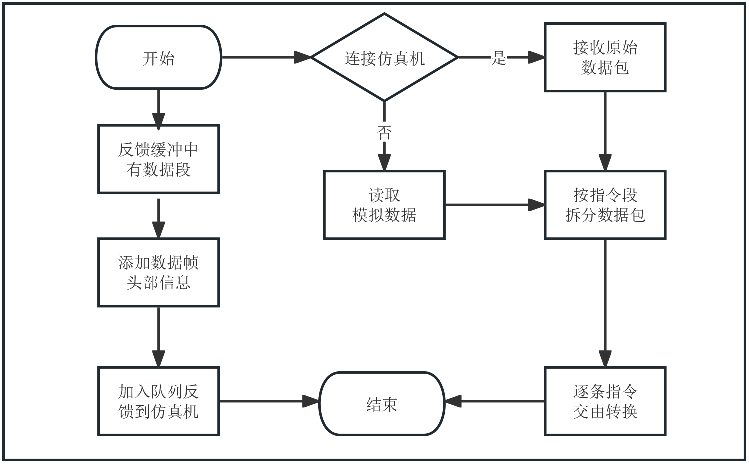
\includegraphics[width=0.8\textwidth]{pictures/flowchart1.pdf}
        \caption{仿真机侧数据交互流程图}
        \label{module11}
    \end{center}
\end{figure}
\subsection{核心类图}
\par
本模块的核心类图如图\ref{module12}所示。其中的核心是类SimulationDeviceContext,它表示仿真机与虚拟仿真机的交流环境
MacLinkCommunication类负责初始化与某一网卡设备的侦听关系,并负责数据帧的实际收取和发送。
MacReceivingRunnable是处理信息收发的线程实例,收取道德数据帧会加入接收数据帧的队列MacReceivingQueueQueue,线程实例从中取数据并交由指令转换模块。
当需要反馈时,线程实例会调用设备实例中的发送方法,最终通过MacLink实现发送。
ISimulatorDeviceInterface代表仿真机设备类的接口,其中包含了对于数据帧中指令代号的读取方法GetSimOperateCode,以及发送消息给仿真机SendToSimulationDevice方法。
CAEGenericSimulatorDeviceBase是该接口的一个实现,其代表CAE公司的仿真机设备,其中含有解读并转换该设备指令的具体算法。当需要接入其他公司设备时,
只需要重新实现SimulatorDevice接口。

\begin{figure}[h!]
    \begin{center}
        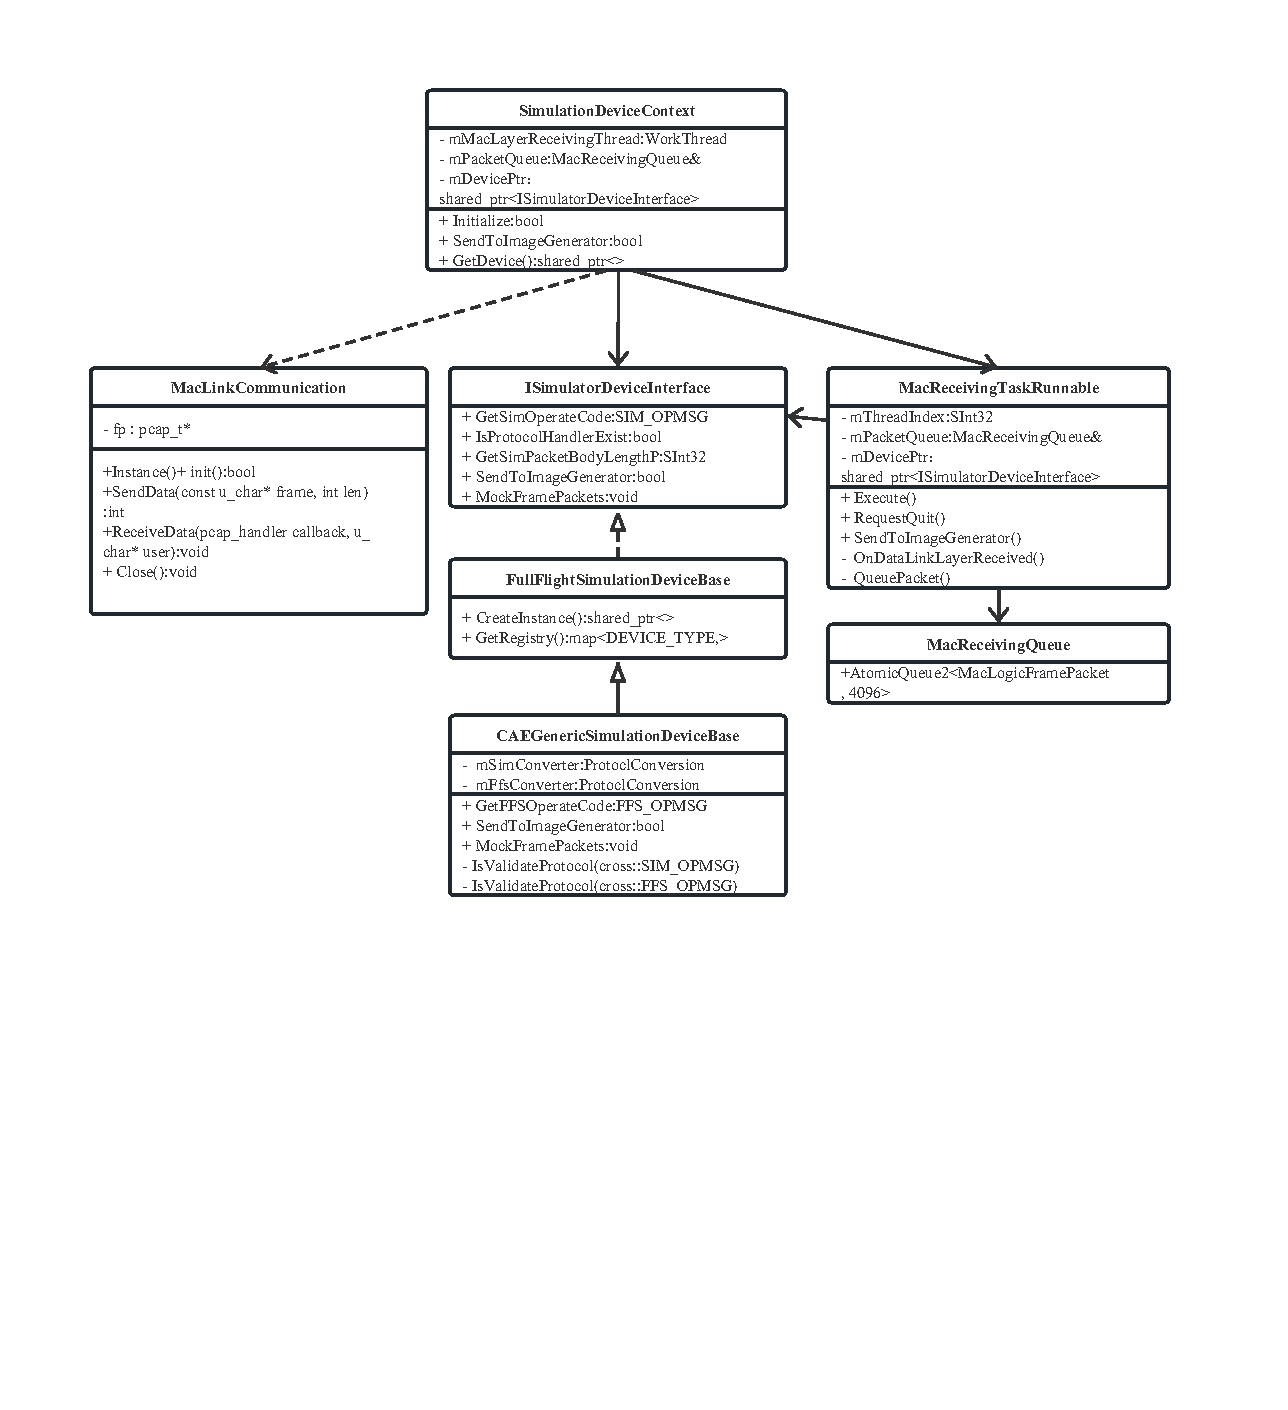
\includegraphics[width=\textwidth]{pictures/classdiagram1.pdf}
        \caption{仿真机侧数据交互核心类图}
        \label{module12}
    \end{center}
\end{figure}
\subsection{顺序图}
图\ref{seq1}是仿真机侧数据交换模块的顺序图,描述了仿真机与虚拟仿真机沟通过程中各类的交互过程。
首先交流环境类SimDeviceContext以mac地址作为参数尝试初始化MacLink,即开始侦听对应网卡设备,MacLink类中利用WinpPcap实现侦听,并判断是否侦听成功。
成功建立连接后,便可以进行数据的收发。交流环境线程MacTaskRunnable运行后会循环执行OnMacRecevied方法,
当有数据到达时会对其进行解封处理并加入MacQueue队列等待指令转换。
但有消息需要反馈时,交流环境调用线程实例的send方法,线程实例调用具体设备实例的send方法,而设备实例最终通过MacLink对象实现发送。
\begin{figure}[h!]
    \begin{center}
        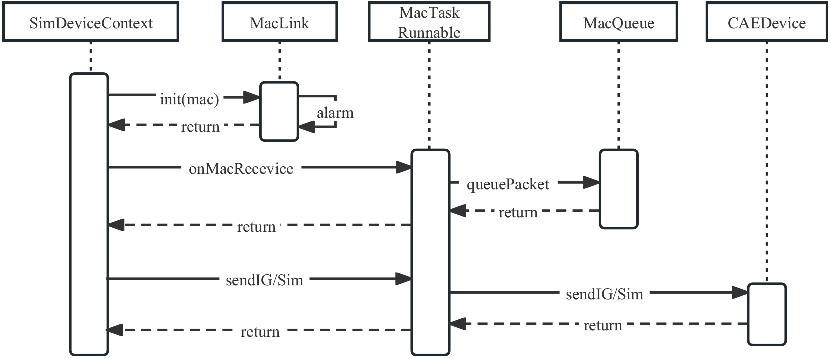
\includegraphics[width=\textwidth]{pictures/sequence1.pdf}
        \caption{仿真机侧数据交换顺序图}
        \label{seq1}
    \end{center}
\end{figure}
\subsection{关键代码}
虚拟仿真机与仿真机间通过数据链路层数据帧直接交换信息,首先要建立连接。类SimulationDeviceContext表示在虚拟仿真机中与仿真机交流的环境,Initialize函数表示了该环境的初始化流程。
代码中用到了条件编译,即根据编译时的参数来编译不同部分的代码。条件MOCKSIM表示是否使用模拟数据。如果编译时带有该参数,那么需要去读取配置文件中的模拟数据文件路径;
否则进一步与真实仿真机建立真实链路层连接。两种方式都需要启动新的线程负责消息的收发工作。
\begin{figure}[h!]
    \centering
     \lstinputlisting[basicstyle= \zihao{6}]{pictures/code1.txt}
    \caption{仿真机环境初始化代码}
    \label{code1}
\end{figure}

\par
真实链路层连接的建立则是使用到WinPcap。在Init方法中,首先通过pcap\_findalldevs方法获得该机器中所有网卡的信息,用户需要根据打印的信息选择需要使用的网卡。
之后使用pcap\_open\_live获得该网卡数据包捕获描述字,成功后即表明完成初始化link layer句柄,虚拟仿真机与仿真机可以通过用户选择的网卡进行交流。
最后通过pcap\_freealldevs释放网卡数据列表。

\begin{figure}[h!]
    \centering
     \lstinputlisting[basicstyle= \zihao{-5}]{pictures/code2.txt}
    \caption{链路层连接建立代码}
    \label{code2}
\end{figure}

\par
WorkerThread是一个由线程定义与线程实例组成的结构体。上文中提到,根据条件编译结果,会得到与仿真机或模拟数据交流的两种线程定义,
CreateRunnableThread负责根据编译情况创建工作线程,图\ref{code3}工作线程mMacLayerThread,作为与仿真机交流环境中的线程。
\begin{figure}[h!]
    \centering
     \lstinputlisting[basicstyle= \zihao{-5}]{pictures/code3.txt}
    \caption{创建工作线程代码}
    \label{code3}
\end{figure}

\par
如图\ref{code4}中第一段代码所示,原始数据包接收线程启动后,会在收到结束请求前循环执行ReceiveData方法收取数据。该方法中含有回调函数OnDataLinkReceived,用于进一步处理接收到的原始数据包,其实现如第二段代码所示。
该回调函数中会将原始数据包中的多条指令拆开,并将每段指令依次存入集合framePackets中。最后调用QueuePacket函数将该集合加入仿真机消息接收队列中。
\begin{figure}[h!]
    \centering
     \lstinputlisting[basicstyle= \zihao{-5}]{pictures/code4.txt}
    \caption{原始数据包接收代码}
    \label{code4}
\end{figure}

\par
如图\ref{code5}所示。原始数据包的解析逻辑位于方法OnDataLinkLayerReceived中。由于原始数据包是数据链路层消息,其带有数据帧头、厂商自定义信息头等数据头部信息,拆分指令段前指针cursor需要先通过ParseMacLinkLayerHeader方法跳过该部分内容,进入正式数据部分。
该部分中含有多条指令,每条指令头部有其长度信息,指针需要按照读取到的长度将数据部分进行拆分,并将指令内容复制到MacEncodingPacket对象中,加入上述仿真机消息接收队列中。虚拟仿真机从仿真机接收消息的过程就此结束。
\par
在真实的飞行训练中虚拟仿真机自然要与仿真机进行直接沟通,但在没有仿真机的开发环境中,虚拟仿真机也需要能够读取模拟数据来驱动视景系统运行。
在编译项目时将条件设置为使用模拟数据,便可以开启该流程。
\par
图\ref{code6}是处理模拟数据的实现。设备指针mDevicePtr调用MockFramePacket方法读取csv文件,ConvertCsv函数将16进制字符两两一组转换为字节内容,最后将读取到的内容转换为MacEncodingPacket类型加入仿真机消息接收队列,此部分与连接仿真机时的过程相同。读取csv文件使用到了第三方库rapidcsv。
NextCurrentFrameMockData方法中指针mCurrentCursor记录了当前读取到的csv文件行数,每次被调用都会从当前位置读取下一行数据内容。
其中,mDocument表示csv文件对象,GetRow方法可以将csv中的一行内容读取到一个vector对象中。随后会根据读取到的指令代号调用相应的转换方法ConvertCsv,把vector对象转换为指令结构体。
\begin{figure}[h!]
    \centering
     \lstinputlisting[basicstyle= \zihao{6}]{pictures/code5.txt}
    \caption{原始数据包解析代码}
    \label{code5}
\end{figure}
\begin{figure}[h!]
    \centering
     \lstinputlisting[basicstyle= \zihao{6}]{pictures/code6.txt}
    \caption{模拟数据处理代码}
    \label{code6}
\end{figure}

\par
第三章需求部分提到,视景系统会给仿真机反馈信息,该消息同样需经过虚拟仿真机,将TCP消息最终转换为原始数据包进行发送。在仿真机交流环境中SendToSimulationDevice方法负责反馈信息,即将指令结构体转换为原始数据包后发送,其调用上文中的工作线程下的同名方法,由该线程负责执行工作。
最终的实现方法则在具体的设备中,因为不同厂商的仿真机使用的数据组织结构大有不同,此处列出了为适配CAE公司仿真机而编写的方法。
\begin{figure}[h!]
    \begin{center}
        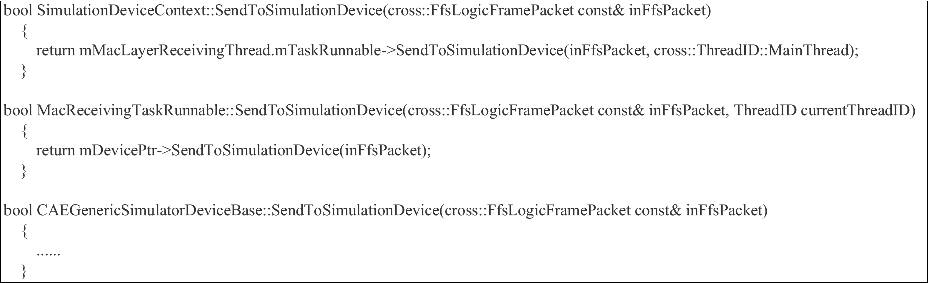
\includegraphics[width=\textwidth]{pictures/code8.pdf}
        \caption{反馈消息逻辑}
    \end{center}
\end{figure}
\par
从视景系统中来的反馈信息类型为FfsLogicFramePacket,需要将其最终封装为数据帧发送。首先需要获取其中的指令代号,调用对应指令的转换方法,若暂时无法理解该指令便产生警告。
其次需要为该数据帧添加仿真机规定的头部和尾部信息,最后通过MacLinkCommunication单例中的SendData完成数据链路层信息的发送。
\par
在使用模拟数据的情况下,如图\ref{feedbackmock}对于信息反馈只要解析其中的指令代号并打印日志即可。
\begin{figure}[h!]
    \begin{center}
        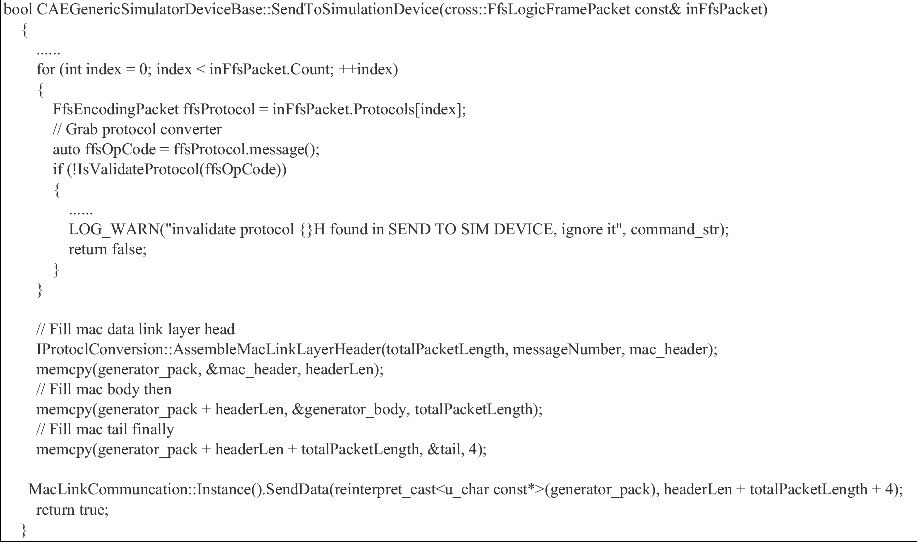
\includegraphics[width=\textwidth]{pictures/code9.pdf}
        \caption{反馈消息实现代码}
    \end{center}
\end{figure}

\begin{figure}[h!]
    \begin{center}
        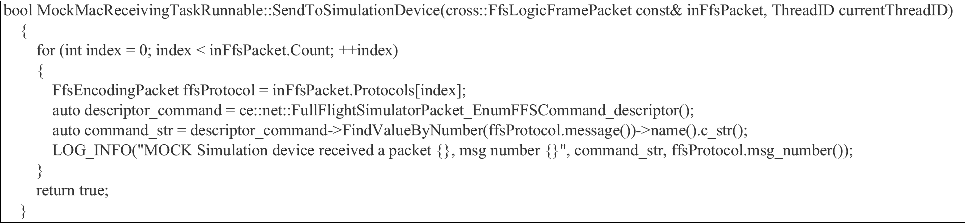
\includegraphics[width=\textwidth]{pictures/code10.pdf}
        \caption{模拟数据下反馈}
        \label{feedbackmock}
    \end{center}
\end{figure}
\par
CAEGenericSimulatorDeviceBase中的构造函数里进行了注册convert
不同厂商的仿真机厂商对于数据包中字段组成和属性编排有明显差异。如表\ref{simsattr}中对比了CAE公司和波音公司模拟机对于飞机移动这一指令数据包中的情况。
通过对比可知,首先他们的头部信息存在差别;其次虽然这一数据包中都含有经纬度、海拔高度和欧拉角信息,但他们的排列顺序明显不同;最后,对于同一个属性如Altitude长度不同,存在精度上的差异。
这些差异最终需要重新解释为统一格式以实现通用化。如图\ref{classtmp}中的代码所示,SD\_PACKET\_21H便是一个统一后用于表示飞机飞行数据的指令结构体。其中包含了基本的飞行用属性。适配新的仿真机只需要重新编写对数据包的解析函数。
\begin{table}[htbp]
    \begin{center}
        \caption{不同仿真机字段比较}
        \label{simsattr}
        \renewcommand\arraystretch{1.2}
        \begin{tabularx}{\textwidth}{ 
            | >{\centering\arraybackslash\hsize=\hsize\linewidth=\hsize}X 
            | >{\centering\arraybackslash\hsize=\hsize\linewidth=\hsize}X 
            | >{\centering\arraybackslash\hsize=\hsize\linewidth=\hsize}X 
            | >{\centering\arraybackslash\hsize=\hsize\linewidth=\hsize}X 
            | }
            \hline
            \textbf{CAE字段} & \textbf{长度} & \textbf{Boeing字段} & \textbf{长度}\\
            \hline
            OpCode & 16bit & Packet ID & 16bit\\
            \hline
            CS number & 32bit & Entity ID & 16bit\\
            \hline
            Latitude MSW & 32bit & Roll & 32bit\\
            \hline
            Latitude LSW & 32bit & Pitch & 32bit\\
            \hline
            Longitude MSW & 32bit & Yaw & 32bit\\
            \hline
            Longitude LSW & 32bit & Latitude MSW & 32bit\\
            \hline
            Altitude& 32bit & Latitude LSW & 32bit\\
            \hline
            Roll & 32bit & Longitude MSW & 32bit\\
            \hline
            Pitch& 32bit & Longitude LSW & 32bit\\
            \hline
            Yaw & 32bit & Altitude & 64bit\\
            \hline
            etc. & & etc. & \\
            \hline
        \end{tabularx}
    \end{center}
\end{table}
\begin{figure}[h!]
    \begin{center}
        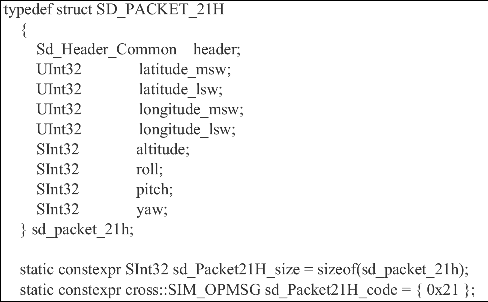
\includegraphics[width=0.8\textwidth]{pictures/code12.pdf}
        \caption{转换类模板代码}
        \label{classtmp}
    \end{center}
\end{figure}

\section{指令转换模块}
指令转换模块负责仿真机指令与自定义指令之间的转换。经过转换后的指令才能被对方理解并使用。首先仿真机指令中对于浮点数的表达方式是由该厂商自行设计的,对于不同用途不同精度要求的数据其数字表示方式均存在差异。
因此这两种结构之间的转换需要严格依照设计文档中的说明设计转换算法,而不是简单的赋值。
其次仿真机指令中最重要的无疑是关于飞机位置和姿态的指令,但由仿真机给出的位置是由经纬度高度组成的数据,而图像生成器中使用的坐标系是笛卡尔坐标系,必须经过坐标系的转换才能使用该信息。
\subsection{流程图}
\par
本模块的主要执行流程如图\ref{module21}所示。
当收到来自仿真机的指令段时,数据转换模块先根据指令代号确定指令类型,用对应的仿真机指令结构体实现反序列化,再根据指令代号查找出对应的转换器,该转换器中的转换方法可将该指令转换为对应的自定义指令。
当收到自定义指令时,同样根据指令类型查找相应的转换器,使用该转换器中的方法完成转换。
\begin{figure}[h!]
    \begin{center}
        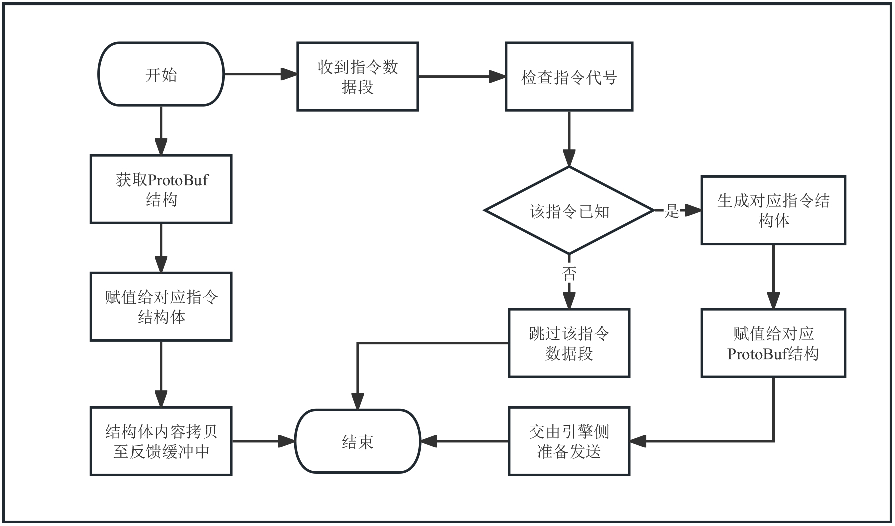
\includegraphics[width=0.8\textwidth]{pictures/flowchart2.pdf}
        \caption{数据转换流程图}
        \label{module21}
    \end{center}
\end{figure}
\subsection{核心类图}
\par
本模块的核心类图如图\ref{module22}所示。其中核心为IProtoclConversion接口,该接口中声明了仿真机指令与自定义指令间转换的方法Convert。需要注意的是在接口的实现中只需要实现其中一个方向的转换,因为一种指令只可能由仿真机给图像生成器或由图像生成器反馈给仿真机。
在CAE仿真机类中使用map存储这些转换器,表示这些转换器是专用于CAE仿真机指令的转换,如果需要接入其他仿真机则需要实现对应的转换器。
ProtoclConversion是一个模板类,成员属性T表示一个仿真机指令,成员属性F表示一个自定义指令,T和F组成互相转换的一对。
IGCommand是自定义指令类,SimCommand是仿真机指令类,真正的Convert实现在仿真机指令类中。
\par
当调用实例化模板类中的Convert方法时,该方法会调用对应指令的Convert方法。
这样设计的原因是当增加仿真机指令类型时不用考虑编写对应的转换器,为协同开发带来便利。

\begin{figure}[h!]
    \begin{center}
        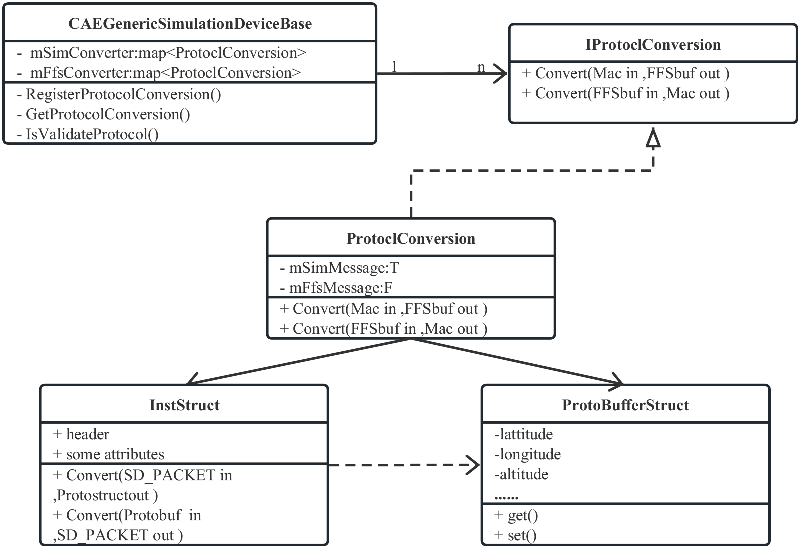
\includegraphics[width=\textwidth]{pictures/classdiagram2.pdf}
        \caption{指令转换核心类图}
        \label{module22}
    \end{center}
\end{figure}
\subsection{顺序图}
图\ref{seq2}是协议转换模块的顺序图。描述了仿真机指令与自定义指令的转换中各类的交互过程。
在系统启动后,CAEDevice的构造函数会完成所有转换器的注册,即将指令代号与指令转换器作为键值对加入map中。
在指令转换前,需要先通过指令代号到map中获取对应的转换器。
调用实例化转换器中的Convert方法时,该方法会调用到仿真机指令中的Convert实现方法。
\begin{figure}[h!]
    \begin{center}
        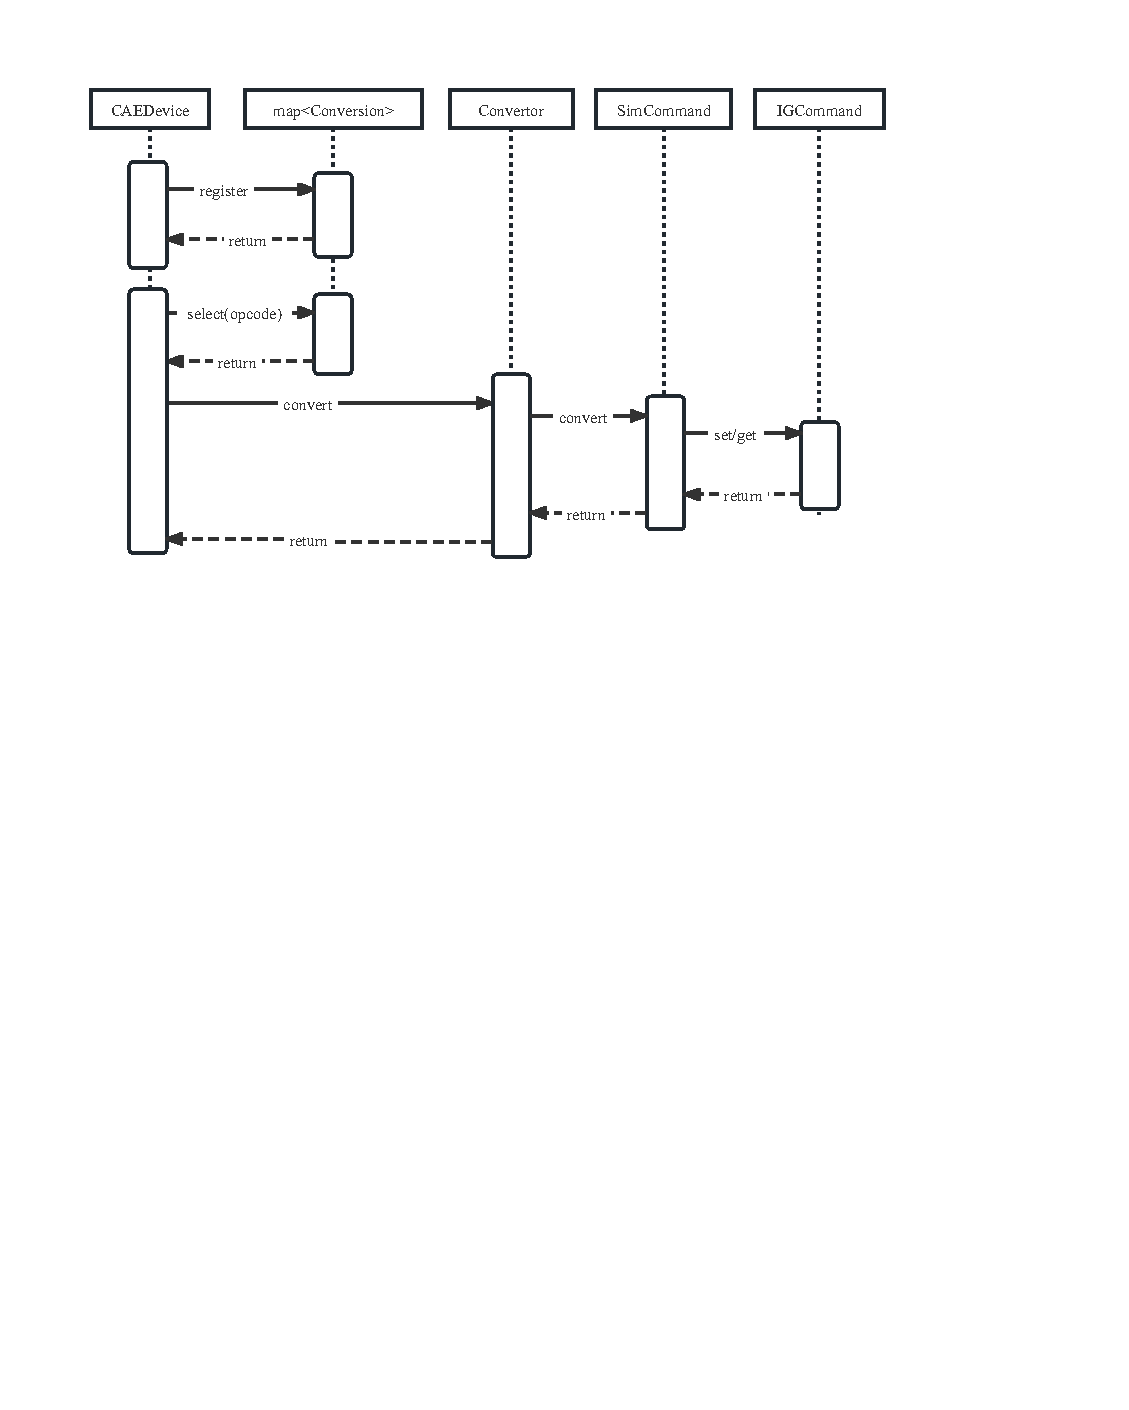
\includegraphics[width=\textwidth]{pictures/sequence2.pdf}
        \caption{指令转换顺序图}
        \label{seq2}
    \end{center}
\end{figure}
\subsection{关键代码}
使用ProtoBuffer首先需要编写一个proto文件定义程序中需要处理的结构化数据,在ProtoBuffer的术语中,结构化数据被称为Message。
如图\ref{pb21}中的代码,定义了一个名为GeodeticCSUpdate的结构化数据,其中的成员为飞机飞行所需属性,且每一个成员均被赋予唯一的编号,在编码时使用该编号表示该成员。

\begin{figure}[h!]
    \begin{center}
        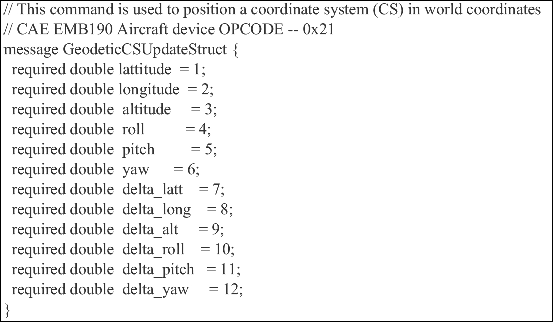
\includegraphics[width=0.8\textwidth]{pictures/code15.pdf}
        \caption{ProtoBuffer结构}
        \label{pb21}
    \end{center}
\end{figure}
\par
写好proto文件之后就可以用ProtoBuffer编译器将该文件编译成目标语言。编译为C++后会得到.pb.h和.pb.cc文件,分别为该类的头文件和实现文件,
提供了一系列的get/set函数用来修改和读取结构化数据中的数据成员。当需要将该结构化数据序列化时,类中已经提供相应的方法来把复杂的数据变成字节序列。
对想要读取数据的程序来说,也只需要使用类中的相应反序列化方法来将这个字节序列重新转换为结构化数据。

\par
系统在需要转换的时候总要根据指令代号来确定对应的转换方法,便要求在系统运作前完成对于这些转换执行者的注册。
如图\ref{convtmp}所示,类ProtoclConversion是转换执行者,这是一个模板类。T代表一个指令结构体,如上文中的SD\_PACKET\_21H;F代表一个ProtoBuffer结构如GeodeticCSUpdate。
如果指令代号为21H,则使用对应的转换执行对象里的Convert方法即可实现转换。
\begin{figure}[h!]
    \begin{center}
        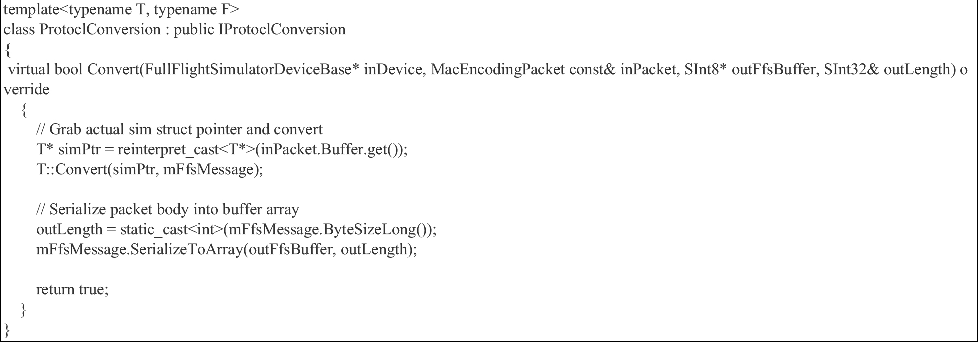
\includegraphics[width=\textwidth]{pictures/code13.pdf}
        \caption{转换执行模板类}
        \label{convtmp}
    \end{center}
\end{figure}
\par
对于一系列ProtoclConversion对象的注册代码如图\ref{regiconv}所示。转换执行者分为两组,一组为mSimConverter,根据仿真机侧的指令代号找到转换执行者;另一组为mFfsConverter,可以根据引擎侧的指令代号找到转换执行者。
RegisterProtocolConversion函数负责将执行者加入两个map中,key为指令代号,value为转换执行者的指针。此函数会在整个环境的构造函数中被多次调用,完成所有注册。
\begin{figure}[h!]
    \begin{center}
        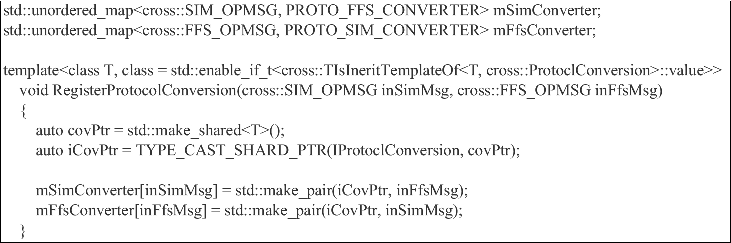
\includegraphics[width=0.9\textwidth]{pictures/code14.pdf}
        \caption{转换执行类注册代码}
        \label{regiconv}
    \end{center}
\end{figure}
\section{图像生成器侧数据交换模块}
游戏引擎侧数据交换模块负责虚拟仿真机与游戏引擎之间的交流。其利用Tbuspp插件使用TCP消息沟通,数据交换协议则是ProtoBuffer。再发送给游戏引擎的过程中,需要将发送频率的固定,因此该线程会以固定的频率被唤醒。
\subsection{流程图}

本模块的主要执行流程如图\ref{module31}所示。当发送队列中有消息时,若可以进行发送则直接发送,否则要等待新的发送时机。反馈消息接收时则不需考虑频率,直接接收消息并给到协议转换模块。
\begin{figure}[h!]
    \begin{center}
        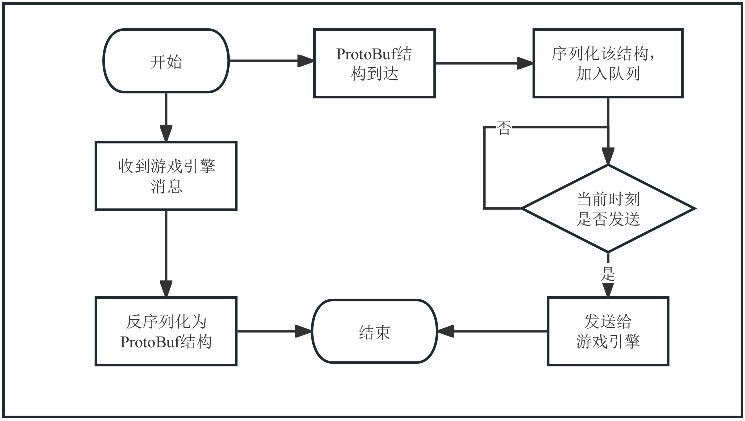
\includegraphics[width=0.8\textwidth]{pictures/flowchart3.pdf}
        \caption{图像生成器侧数据交互流程图}
        \label{module31}
    \end{center}
\end{figure}
\subsection{核心类图}

本模块的核心类图如图\ref{module32}所示。其中的核心是类ImageGeneratorContext,它表示在虚拟仿真机中与游戏引擎交流的环境,其中包含控制信息收发的线程和信息队列。
IImageGeneratorDeviceInterface则是与游戏引擎交流的接口,其中包含了对于ProtoBuffer结构中指令代号的读取方法GetOperateCode,以及发送消息给游戏引擎SendToImageGenerator方法。
FullFightSimulatorDeviceBase是对该接口的实现,其依赖控制发送频率的类FrameSynchronization。CAEGenericSimulatorDeviceBase代表CAE公司FFS设备,其中含有与该公司设备进行沟通的具体方法。
\begin{figure}[h!]
    \begin{center}
        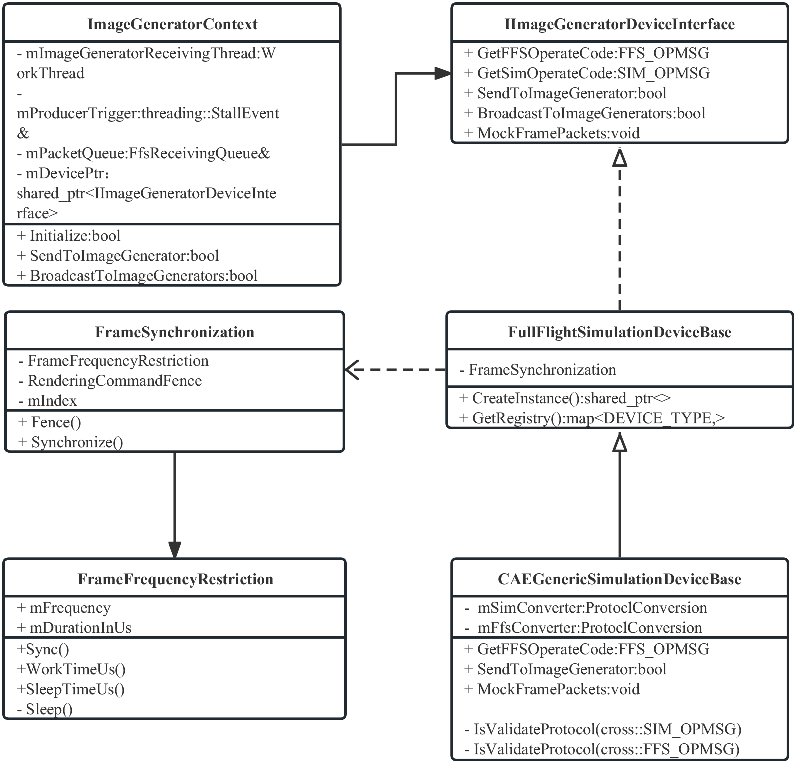
\includegraphics[width=\textwidth]{pictures/classdiagram3.pdf}
        \caption{视景系统侧数据交互核心类图}
        \label{module32}
    \end{center}
\end{figure}
\subsection{顺序图}
图\ref{seq3}是游戏引擎侧数据交换模块的顺序图。描述了虚拟仿真机与游戏引擎间沟通时各类的交互过程。
首先交流环境IGContext先通过Tbuspp的配置文件建立连接,Tbuspp插件类会判断连接是否成功。
连接建立后,交流环境通过send方法通知FFSDevice已有数据准备好发送,此时FrameSync类会介入判断在规定发送频率下此时是否可以发送。
到达发送时间后,会调用IGDevice中的send方法执行具体发送动作。
\begin{figure}[h!]
    \begin{center}
        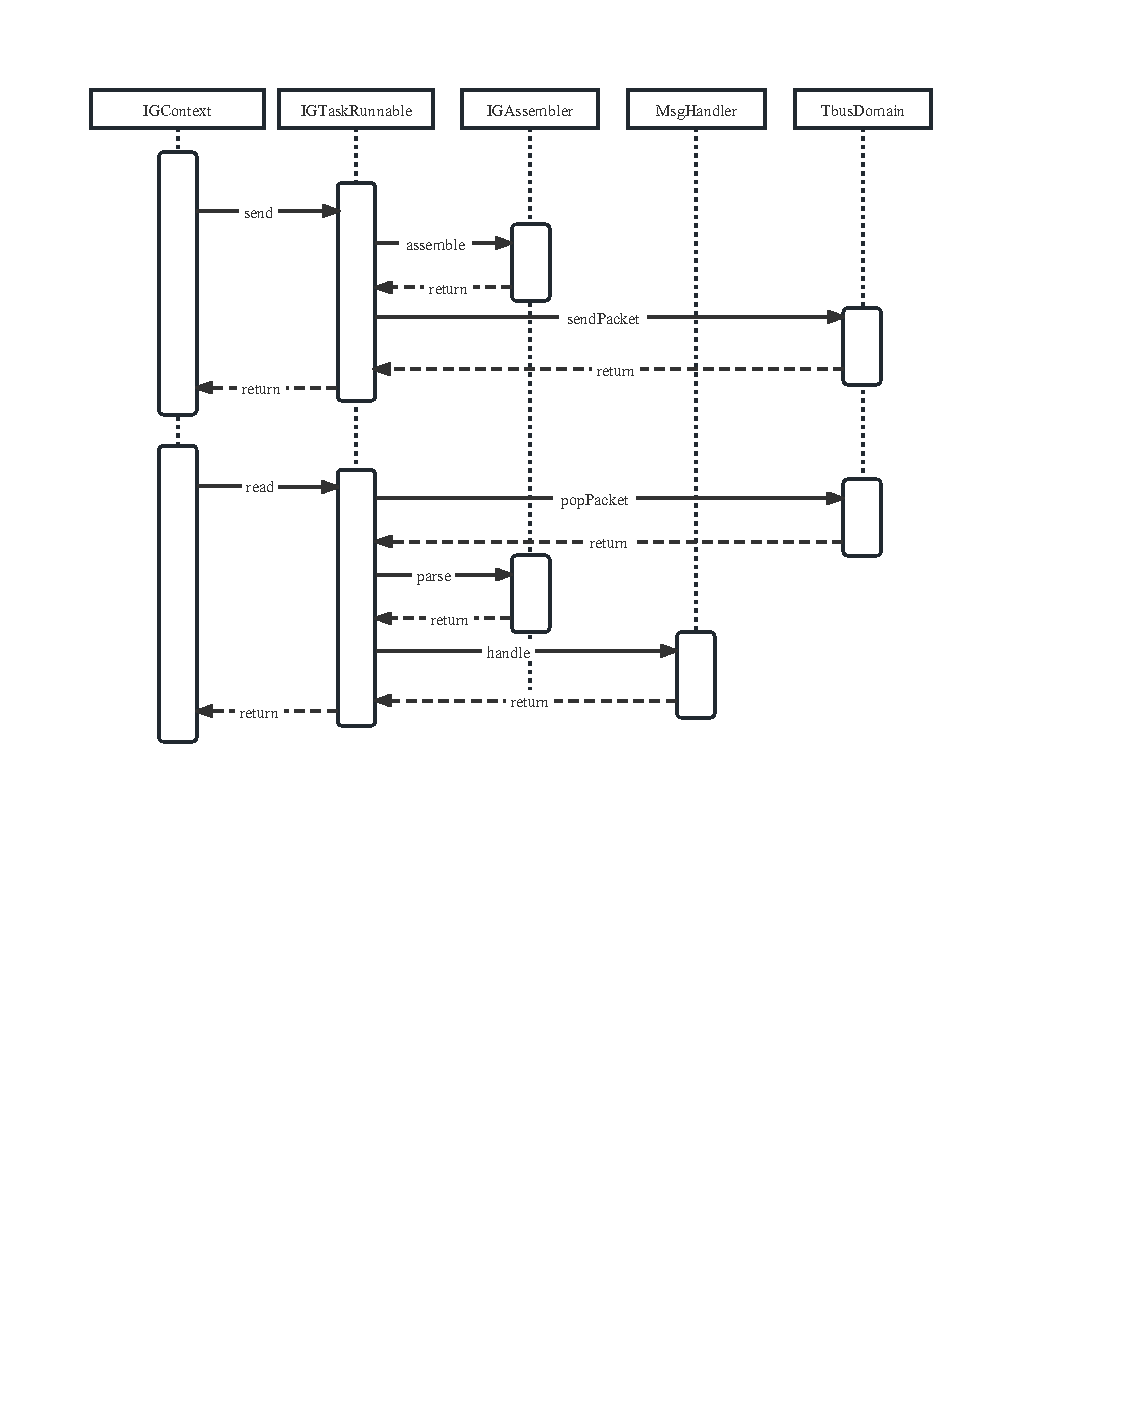
\includegraphics[width=\textwidth]{pictures/sequence3.pdf}
        \caption{游戏引擎侧数据交换顺序图}
        \label{seq3}
    \end{center}
\end{figure}
\subsection{关键代码}
虚拟仿真机与游戏引擎之间通过Tbuspp插件进行信息交流,第一步是要先建立连接。类ImageGeneratorContext表示在虚拟仿真机中与游戏引擎交流的环境,Initialize函数表示了该环境的初始化流程。
代码中同样用到了条件编译。条件MOCKIG表示不与游戏引擎建立真实连接,而是直接读取配置文件中的模拟数据文件路径,模仿视景系统给到的反馈,暂时该功能并未投入使用;
否则进一步与游戏引擎建立连接。两种方式都需要启动新的线程负责消息的收发工作。
\begin{figure}[h!]
    \begin{center}
        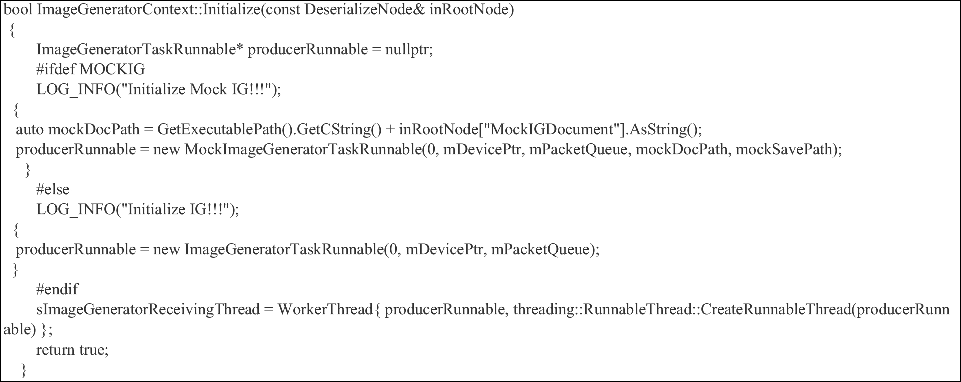
\includegraphics[width=0.9\textwidth]{pictures/code17.pdf}
        \caption{引擎侧环境初始化代码}
    \end{center}
\end{figure}
\par
Tbuspp连接的建立首先需要编写一个简单的配置文件,其中需要给出每个节点的url和busid。如图\ref{tbusconfi}中所示,VSD节点表示虚拟仿真机,另外还包含有两个视景节点,ImageGeneratorGroup则代表所有的视景节点,
当需要广播消息时可以给到该节点。此处的url均为本地地址,实际运行中,虚拟仿真机与视景系统运行在不同机器上,需根据实际情况进行配置。
\par
在Tbuspp初始化方法中,node参数表示已经过反序列化的配置文件内容,首先通过LoadDomainConfig读取所有的节点;其次通过SetLocalClient设置本地的服务节点,在虚拟仿真及侧该节点为VSD。之后使用tbuspp\_open方法开启连接,
并检查连接状态是否正常。随后获取消息的接收和发送队列in\_queue和out\_queue并对他们进行一次清空操作,做好收发消息的准备。

\begin{figure}[h!]
    \begin{center}
        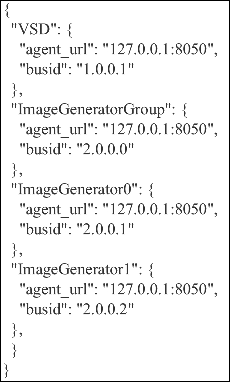
\includegraphics[width=0.3\textwidth]{pictures/code18.pdf}
        \caption{Tbuspp配置文件}
        \label{tbusconfi}
    \end{center}
\end{figure}
\begin{figure}[h!]
    \begin{center}
        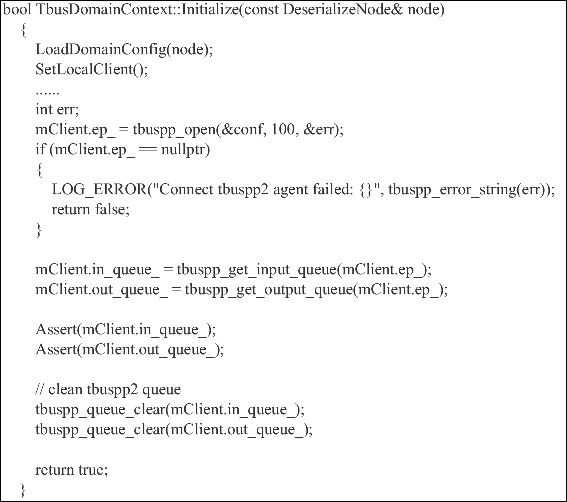
\includegraphics[width=0.8\textwidth]{pictures/code19.pdf}
        \caption{Tbuspp初始化代码}
    \end{center}
\end{figure}
\par
SendToImageGenerator方法负责发送信息至游戏引擎。其参数包括需要发送的数据和接收数据的视景系统节点名称。使用SerializeToArray方法对待发送数据进行序列化后,便交由TbusDomainContext单例处理发送操作。
其中先根据节点名称确定发送的目标节点,之后通过tbuspp\_queue\_write方法将发送内容写入本地服务节点的发送队列out\_queue中,由Tbuspp完成发送。
\begin{figure}[h!]
    \begin{center}
        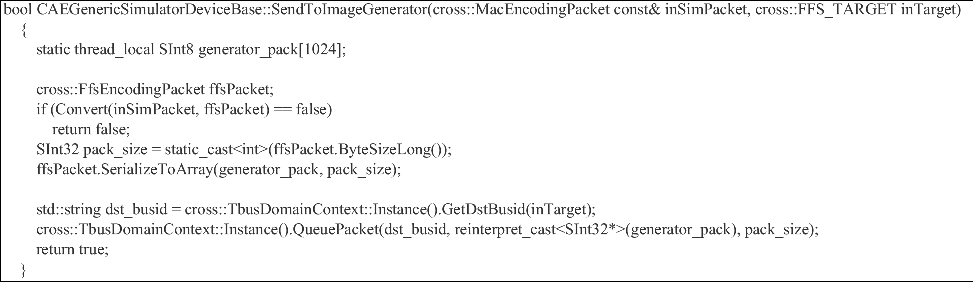
\includegraphics[width=0.9\textwidth]{pictures/code20.pdf}
        \caption{引擎侧发送信息代码}
    \end{center}
\end{figure}
\begin{figure}[h!]
    \begin{center}
        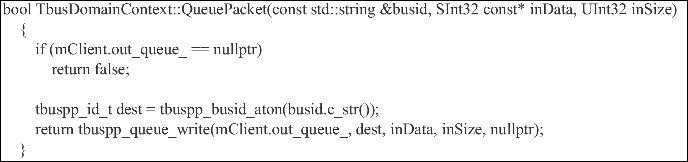
\includegraphics[width=0.8\textwidth]{pictures/code21.pdf}
        \caption{Tbuspp发送信息代码}
    \end{center}
\end{figure}
\par
在游戏中逻辑线程负责数据的产生,渲染线程负责根据数据渲染画面,一般比逻辑线程慢许多。因为逻辑线程跑的太快基本没有意义,还会耗光内存。因为逻辑线程不断的产生数据传递给渲染线程,如果渲染线程消费数据远远慢于产生数据,就会有越来越多的数据存于内存中。
因此需要对逻辑线程做出一定限制,不能让其一直保持工作状态。
\par
在本系统中对于仿真机数据的处理和传输可以认为是逻辑线程的工作,而游戏引擎部分基本为渲染线程的工作。图\ref{sync}是对于逻辑线程进行限制的核心方法Sync。
high\_resolution\_clock是C++11中的新特性,提供的拥有最小计次周期的时钟。在本系统中以微妙作为基本周期,FrameDurationUs表示每次发送的间隔周期,如果要求为60Hz的发送频率则该值为$10^6/60$微秒。
若距离上一次发送的时间仍小于间隔周期,则使用Sleep方法将线程挂起剩余的时间长度。
\begin{figure}[h!]
    \begin{center}
        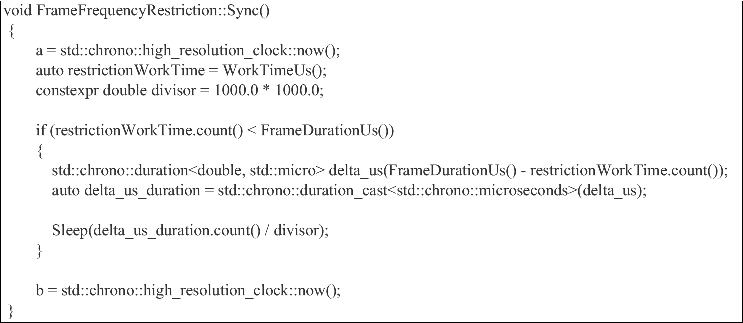
\includegraphics[width=0.8\textwidth]{pictures/code22.pdf}
        \caption{限制频率代码}
        \label{sync}
    \end{center}
\end{figure}
\par
在第二章的介绍中提到Nagle算法可以减少TCP包的个数,更高效的利用网络带宽。但同时也会带来一些延时问题,在实时交互应用中尤其重要。
对于部署虚拟仿真机和游戏引擎的Windows系统机器都需要在注册表中将TcpAckFrequency字段和TcpNoDelay字段值修改为1,以禁用Nagle算法。
\begin{figure}[h!]
    \begin{center}
        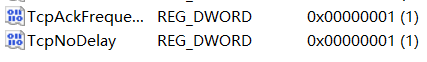
\includegraphics[width=0.8\textwidth]{pictures/nagle.png}
        \caption{Windows中禁用Nagle}
    \end{center}
\end{figure}
\section{飞行控制模块}
\subsection{顺序图}
图\ref{seq4}是飞行控制模块的顺序图,描述了游戏引擎执行飞行逻辑时各类大致的交互过程。
场景类World每帧调用tick函数执行该帧中的操作,逻辑脚本FlightScript调用引擎核心中负责变换和物理的System中的算法,完成飞机的移动旋转,以及对于下方地形的检测。
Camera类也会被World每帧调用,执行不同视角逻辑下的移动旋转,变焦等动作。
\begin{figure}[h!]
    \begin{center}
        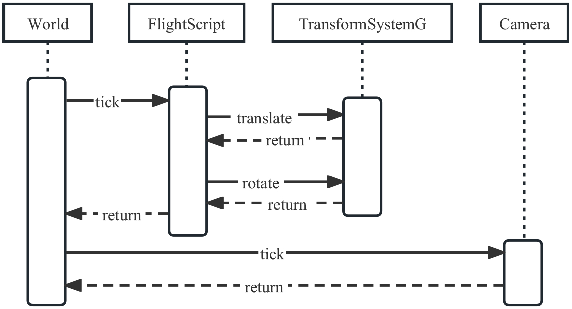
\includegraphics[width=.8\textwidth]{pictures/sequence4.pdf}
        \caption{飞行控制顺序图}
        \label{seq4}
    \end{center}
\end{figure}
\subsection{飞行位置与姿态计算}
由经度longitude,纬度latitude和高度altitude组成的LLA坐标系,可以说是最为广泛应用的一个地球坐标系,它给出一点的大地纬度、大地经度和大地高程直观地告诉我们该点在地球中的位置,故又被称作经纬高坐标系。仿真机给出的飞机位置便是LLA坐标形式。
地心地固坐标系ECEF是以地心为原点的笛卡尔坐标系,在游戏引擎中自然使用该坐标系更为便捷。在两种坐标系下地球都是默认为两级略扁的规则椭球形,赤道长半轴为6378137.0米,两极短半轴为6356752.314245米,扁率为1/298.257223563。
B. R. Bowring在1985年便提出了两种坐标间的转换方法\cite{cha4}。如图\ref{lla2ecef}和图\ref{ecef2lla}所示。其中a为长半轴,b为短半轴,e为椭球的偏心率,N为椭球的曲率半径。
$$e^2=\frac{a^2-b^2}{a^2}$$
$$N=\frac{a}{\sqrt{1-e^2sin^2(lat)}}$$

\begin{figure}[h!]
    \begin{center}
        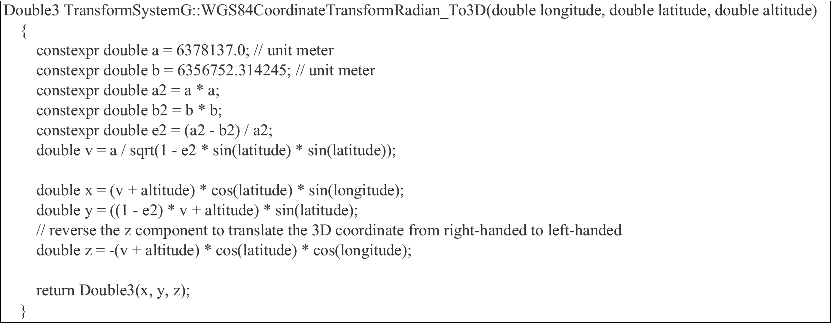
\includegraphics[width=0.8\textwidth]{pictures/code23.pdf}
        \caption{LLA转换为ECEF坐标代码}
        \label{lla2ecef}
    \end{center}
\end{figure}

\begin{figure}[h!]
    \begin{center}
        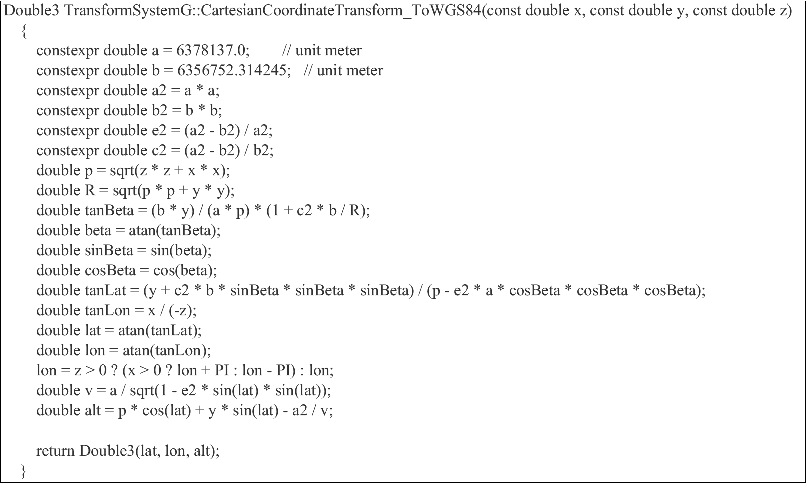
\includegraphics[width=0.8\textwidth]{pictures/code28.pdf}
        \caption{ECEF转换为LLA坐标代码}
        \label{ecef2lla}
    \end{center}
\end{figure}
\par 
除了LLA与ECEF之间的转换,我们还需要建立一个东北天坐标系ENU,这是一个在物体所在位置建立的坐标系,三个轴分别指向东方,上方和北方。飞机的欧拉角便是以ENU坐标系为初始状态进行旋转。
我们依旧可以仅从LLA坐标得到ENU坐标系。如图\ref{llanue}所示,我们可以根据经度和纬度做简单的三角函数运算得出该点法线向量normal,即ENU坐标系中的up方向。同时法线与y轴所构成的平面一定与东方向垂直。
在三维向量下,两个不平行的向量进行叉乘可以得到垂直于该平面的一个向量。根据该几何意义,将normal与y轴单位向量(0,1,0)叉乘即可得到东方向。同理将东方向与normal叉乘,即可得到北方向,ENU坐标系就此构建完毕。
飞机的姿态需要使用欧拉角与ENU坐标系形成的旋转矩阵相乘,才能正确得到游戏引擎世界坐标系ECEF下的姿态。
$$normal.x=cos(lat) * sin(lon)$$
$$normal.y = sin(lat)$$
$$normal.z = -cos(lat) * cos(lon)$$
\begin{figure}[h!]
    \begin{center}
        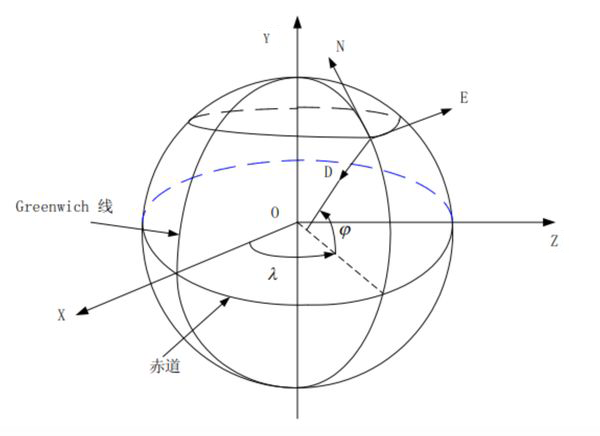
\includegraphics[width=0.8\textwidth]{pictures/ecef.png}
        \caption{LLA与ENU坐标系}
        \label{llaneu}
    \end{center}
\end{figure}



\section{初步运行测试}
\section{本章小结}
本章在需求分析及总体设计的基础上,对系统包含的四个模块核心功能的实现做了具体阐述。对于虚拟仿真机与仿真机和游戏引擎的数据交换模块,都介绍了建立连接的过程和收发信息的过程。仿真机侧额外介绍了为应对不同厂商模拟机而做的设计,
游戏引擎侧则额外介绍了稳定信息收发帧率的实现方法。在协议转换模块中介绍了使用ProtoBuffer协议的流程方法,对较为特殊的字段转换算法做了详细说明。在最后的飞行控制模块中,介绍了让飞机飞行的实现,三种观察方式摄像机的实现,以及飞行中对于地形信息检测的实现。